\chapter*{Resumen}


\chapter{Propuesta} \label{sec:propuesta}

A continuación presentaremos la propuesta técnica del trabajo que usaremos para la elaboración de este sistema de interoperativilidad con SIMBA. Así mismo las herramientas a utilizar y el impacto tecnológico que traerá esto apara el estado de Chiapas. Además la metodología de desarrollo que implementaremos y su justificación de la misma.

\section{Propuesta Técnica}

\begin{figure}[h]
  \label{propuesta}
  \centering
  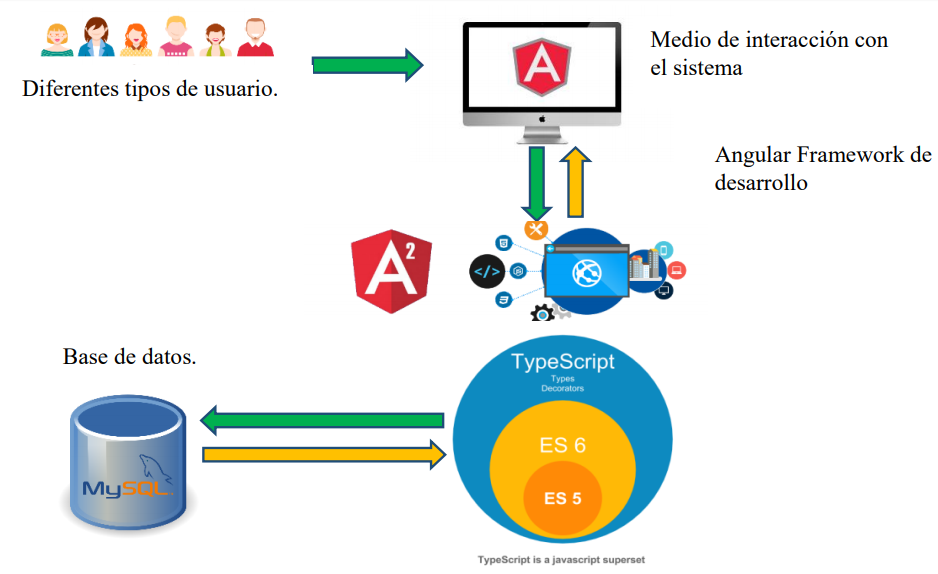
\includegraphics[scale=.4]{lib/assets/propuesta-tecnica}
  \caption{Propuesta Técnica}
\end{figure}


\section{Impácto}

\subsection{Impácto Social}

Según estimaciones oficiales, la aplicación del ECE podría representar el ahorro de 38 mil millones de pesos para el sistema de salud, debido a que se contrarrestarían posibles negligencias médicas, retrasos en la atención, cirugías, robo y desperdicio de medicamento, entre otros. Esto debido a que la falta de información clínica retrasa la atención y puede ser la causa de errores médicos. Esta evolución tecnológica permitirá aumentar la productividad en 20 por ciento; reducir los tiempos y días de espera para consultar en 60 por ciento y ahorros de hasta el 80 por ciento en papelería; reducir los tiempos para cirugía que llegan a ser de hasta 62 días, así como disminuir el desperdicio de medicamento. Además de colocar a México a la altura de otros países que ya implementan este mecanismo. Manual del Expediente Clínico Electrónico. Dirección General de Información en Salud. Secretaría de Salud. México, 2011.
Pacientes con estabilidad respiratoria, hemodinámica y neurológica, el tiempo de espera máximo debe ser de 60 minutos; y verde, pacientes con estabilidad respiratoria, hemodinámica y neurológica, con aspecto saludable y sin riesgo evidente de complicaciones, el tiempo de espera es de hasta cuatro horas. (Chiapas, 2017)
La implementación de un expediente clínico en el estado de Chiapas representaría un gran ahorro económico, tiempo y así como agilizar la atención de cada uno de los pacientes. Actualmente el tiempo de espera para los pacientes en los hospitales llega a ser de cuatro horas, siendo este demasiado tiempo, el cual las personas pudiesen ocupar para realizar sus actividades económicas ya que en el estado un gran porcentaje de la población vive al día con lo poco que gana durante una jornada laborar, siendo esta de una ganancia no estable. Se espera reducir el tiempo de espera en un 80\% con el expediente clínico electrónico.

\subsection{Impácto Tecnológico}
El impácto Tecnológico principal del proyecto será que se desarrolle a las necesidades de la secretaria de salud del estado de Chiapas, siendo una de estas que funcione de manera online y offline, además que pueda contar con una gran escalabilidad ya que es pensado para manejar grandes cantidades de información, datos estadísticos y por supuesto con la mayor seguridad posible.  Con ello se pretende eliminar en su mayoría la duplicidad de los datos o la perdida da de los mismos. Además, se ayudará a aplicar acciones preventivas en la población. Se tendrá un acceso más rápido a la información para la ayuda de investigaciones y desarrollo de la salud en el estado.

\section{Metodología en cascada}
    \subsection{Descripción de la metodología}
      Es el enfoque metodológico que ordena rigurosamente las etapas del ciclo de vida
      del software, de tal forma que el inicio de cada etapa debe esperar a la finalización
      de la inmediatamente anterior (Figura \ref{metodologia})

      \begin{figure}[h]
        \centering
        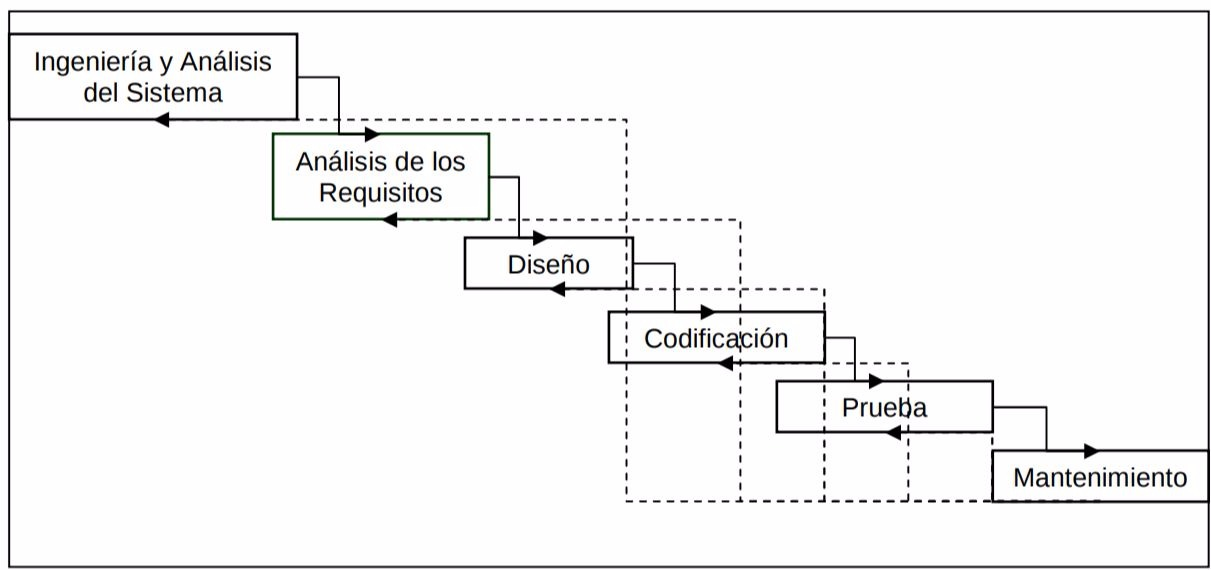
\includegraphics[scale=.3]{lib/assets/diagramaMetodologia}
        \caption{Diagrama de la metodología.}
        \label{metodologia}
      \end{figure}


De esta forma, cualquier error de diseño detectado en la etapa de prueba conduce
necesariamente al rediseño y nueva programación del código afectado, aumentando
los costos del desarrollo.


  \subsection{Justificación de metodología}

  La decisión por el cual se eligió esta metodología fue por la menera en la que se está trabajando con los contribuyentes exteriores, de parte de Secretaria de Salud recibimos la parte de analizis y requerimientos del sistema, por nuestra parte trabajaremos lo que es la interoperabilidad de los Sistemas de expediente Clínico.
        \subsection{Pasos de la metodología}
            \subsubsection{Ingeniería y Análisis del Sistema}
            Debido a que el software es siempre parte de un sistema mayor el trabajo comienza estableciendo los requisitos de todos los elementos del sistema y luego asignando algún subconjunto de estos requisitos al software.
            \subsubsection{Análisis de los requisitos del software}
            El proceso de recopilación de los requisitos se centra e intensifica especialmente en el software. El ingeniero de software (Analistas) debe comprender el ámbito de la información del software, así como la función, el rendimiento y las interfaces requeridas.
            \subsubsection{Diseño}
            El diseño del software se enfoca en cuatro atributos distintos del programa: la estructura de los datos, la arquitectura del software, el detalle procedimental y la caracterización de la interfaz. El proceso de diseño traduce los requisitos en una representación del software con la calidad requerida antes de que comience la codificación.
            \subsubsection{Codificación}
            El diseño debe traducirse en una forma legible para la maquina. El paso de codificación realiza esta tarea. Si el diseño se realiza de una manera detallada la codificación puede realizarse mecánicamente.
            \subsubsection{Pruebas}
            Una vez que se ha generado el código comienza la prueba del programa. La prueba se centra en la lógica interna del software, y en las funciones externas, realizando
            \subsubsection{Mantenimiento}
            E software sufrirá cambios después de que se entrega al cliente. Los cambios ocurrirán debido a que hayan encontrado errores, a que el software deba adaptarse a cambios del entorno externo (sistema operativo o dispositivos periféricos), o debido a que el cliente requiera ampliaciones funcionales o del rendimiento.

    \subsection{Pasos de la metodología aplicada en el proyecto}
          \subsubsection{Ingeniería y Análisis del Sistema}
          \subsubsection{Análisis de los requisitos del software}
          \subsubsection{Diseño}
          \subsubsection{Codificación}
          \subsubsection{Pruebas}
          \subsubsection{Mantenimiento}
